\section{Thống kê mô tả}

    \subsection{Thông tin tổng quát về các biến của bộ dữ liệu}
        Bộ dữ liệu sau khi tiền xử lý bao gồm 9 thông số kỹ thuật phần cứng cốt lõi ảnh hưởng đến hiệu năng của GPU. Dưới đây là bảng mô tả chi tiết kiểu biến, đơn vị đo lường và ý nghĩa của các biến chính:

        \begin{table}[H]
            \centering
            \renewcommand{\arraystretch}{1.3}
            \begin{tabular}{|l|l|c|p{6.2cm}|}
                \hline
                \textbf{Tên biến} & \textbf{Kiểu biến} & \textbf{Đơn vị} & \textbf{Mô tả \& Ý nghĩa} \\
                \hline
                \texttt{Core\_Speed} & Liên tục & MHz & Tốc độ xử lý xung nhịp của GPU, thể hiện số chu kỳ thực hiện được trong 1 giây. \\
                \hline
                \texttt{Memory} & Liên tục & MB & Dung lượng bộ nhớ VRAM của GPU, dùng để lưu trữ dữ liệu và tài nguyên đồ họa. \\
                \hline
                \texttt{Memory\_Bus} & Liên tục & Bit & Độ rộng kênh truyền dẫn dữ liệu giữa bộ nhớ VRAM và các nhân xử lý của GPU. \\
                \hline
                \texttt{Max\_Power} & Liên tục & W & Công suất tiêu thụ tối đa (TDP), thể hiện giới hạn năng lượng cung cấp cho card đồ họa. \\
                \hline
                \texttt{Memory\_Bandwidth} & Liên tục & GB/s & Băng thông bộ nhớ, thể hiện tốc độ truyền tải dữ liệu tối đa giữa GPU và bộ nhớ. \\
                \hline
                \texttt{Memory\_Speed} & Liên tục & MHz & Tốc độ xung nhịp hoạt động của bộ nhớ RAM trên GPU. \\
                \hline
                \texttt{Process} & Liên tục & nm & Tiến trình công nghệ bán dẫn (nanometer) sử dụng trong quá trình chế tạo chip GPU. \\
                \hline
                \texttt{ROPs} & Liên tục & Đơn vị & Số đơn vị xuất kết xuất (Raster Operations Pipelines), xử lý pixel cuối cùng trước khi xuất ra màn hình. \\
                \hline
                \texttt{TMUs} & Liên tục & Đơn vị & Số đơn vị ánh xạ vân bề mặt (Texture Mapping Units), chịu trách nhiệm xử lý và lọc texture. \\
                \hline
            \end{tabular}
            \caption{Thông tin tổng quát về các biến trong bộ dữ liệu GPU}
            \label{tab:thong_tin_bien}
        \end{table}

    \subsection{Bảng các đặc trưng thống kê mô tả}
        Để có cái nhìn định lượng tổng quan về xu hướng tập trung và mức độ phân tán của từng thông số kỹ thuật trước khi biến đổi logarit, nhóm tính toán các tham số thống kê mô tả cơ bản trên tập dữ liệu sạch (kết quả trích xuất từ tệp \texttt{summary\_stats.csv} sau khi chạy lại quy trình tiền xử lý mới):

        \begin{table}[H]
            \centering
            \footnotesize
            \renewcommand{\arraystretch}{1.35}
            \begin{tabular}{|l|c|r|r|r|r|r|r|r|r|}
                \hline
                \textbf{Tên biến} & \textbf{Đơn vị} & \textbf{$N$} & \textbf{Mean} & \textbf{SD} & \textbf{Min} & \textbf{$Q_1$} & \textbf{Median} & \textbf{$Q_3$} & \textbf{Max} \\
                \hline
                \texttt{Core\_Speed} & MHz & 2018 & 982.22 & 256.27 & 200.00 & 800.00 & 1000.00 & 1118.50 & 1784.00 \\
                \hline
                \texttt{Max\_Power} & W & 2018 & 143.36 & 103.73 & 1.00 & 65.00 & 122.00 & 190.00 & 780.00 \\
                \hline
                \texttt{Memory} & MB & 2018 & 3301.90 & 2762.80 & 128.00 & 1280.00 & 2048.00 & 4096.00 & 24576.00 \\
                \hline
                \texttt{Memory\_Bandwidth} & GB/s & 2018 & 164.69 & 137.63 & 4.00 & 70.80 & 128.00 & 224.40 & 1280.00 \\
                \hline
                \texttt{Memory\_Bus} & Bit & 2018 & 223.11 & 247.13 & 64.00 & 128.00 & 192.00 & 256.00 & 4096.00 \\
                \hline
                \texttt{Memory\_Speed} & MHz & 2018 & 1310.03 & 386.16 & 400.00 & 1000.00 & 1350.00 & 1653.00 & 2127.00 \\
                \hline
                \texttt{Process} & nm & 2018 & 30.18 & 10.49 & 14.00 & 28.00 & 28.00 & 40.00 & 90.00 \\
                \hline
                \texttt{ROPs} & Đơn vị & 2018 & 33.93 & 27.82 & 2.00 & 16.00 & 32.00 & 48.00 & 192.00 \\
                \hline
                \texttt{TMUs} & Đơn vị & 2018 & 76.73 & 55.61 & 4.00 & 32.00 & 64.00 & 112.00 & 384.00 \\
                \hline
            \end{tabular}
            \caption{Bảng các đặc trưng thống kê mô tả của 9 biến thông số kỹ thuật GPU}
            \label{tab:dac_trung_thong_ke}
        \end{table}

        \textbf{Nhận xét từ bảng số liệu:}
        \begin{itemize}
            \item Sự chênh lệch lớn giữa giá trị trung bình (\texttt{Mean}) và trung vị (\texttt{Median}), cùng với khoảng cách rất rộng từ tứ phân vị thứ ba ($Q_3$) đến giá trị cực đại (\texttt{Max}) ở các biến như \texttt{Memory}, \texttt{Memory\_Bandwidth}, \texttt{Max\_Power}, \texttt{ROPs}, và \texttt{TMUs} cho thấy dữ liệu có độ phân tán cao và bị lệch phải mạnh.
            \item Việc thực hiện phép chuyển đổi logarit ở bước tiếp theo là hoàn toàn cần thiết để thu hẹp khoảng biến thiên và giảm ảnh hưởng của các giá trị cực đại.
        \end{itemize}

    \subsection{Biểu đồ - đồ thị}
        \subsubsection{Biểu đồ phân bố tần suất (Histogram)}
            Dưới đây là biểu đồ phân bố tần suất cho các biến thông số kỹ thuật phần cứng của GPU trước và sau khi thực hiện phép biến đổi logarit (được vẽ bằng thư viện \texttt{ggplot2} và \texttt{gridExtra} trong R):

            \begin{figure}[H]
                \centering
                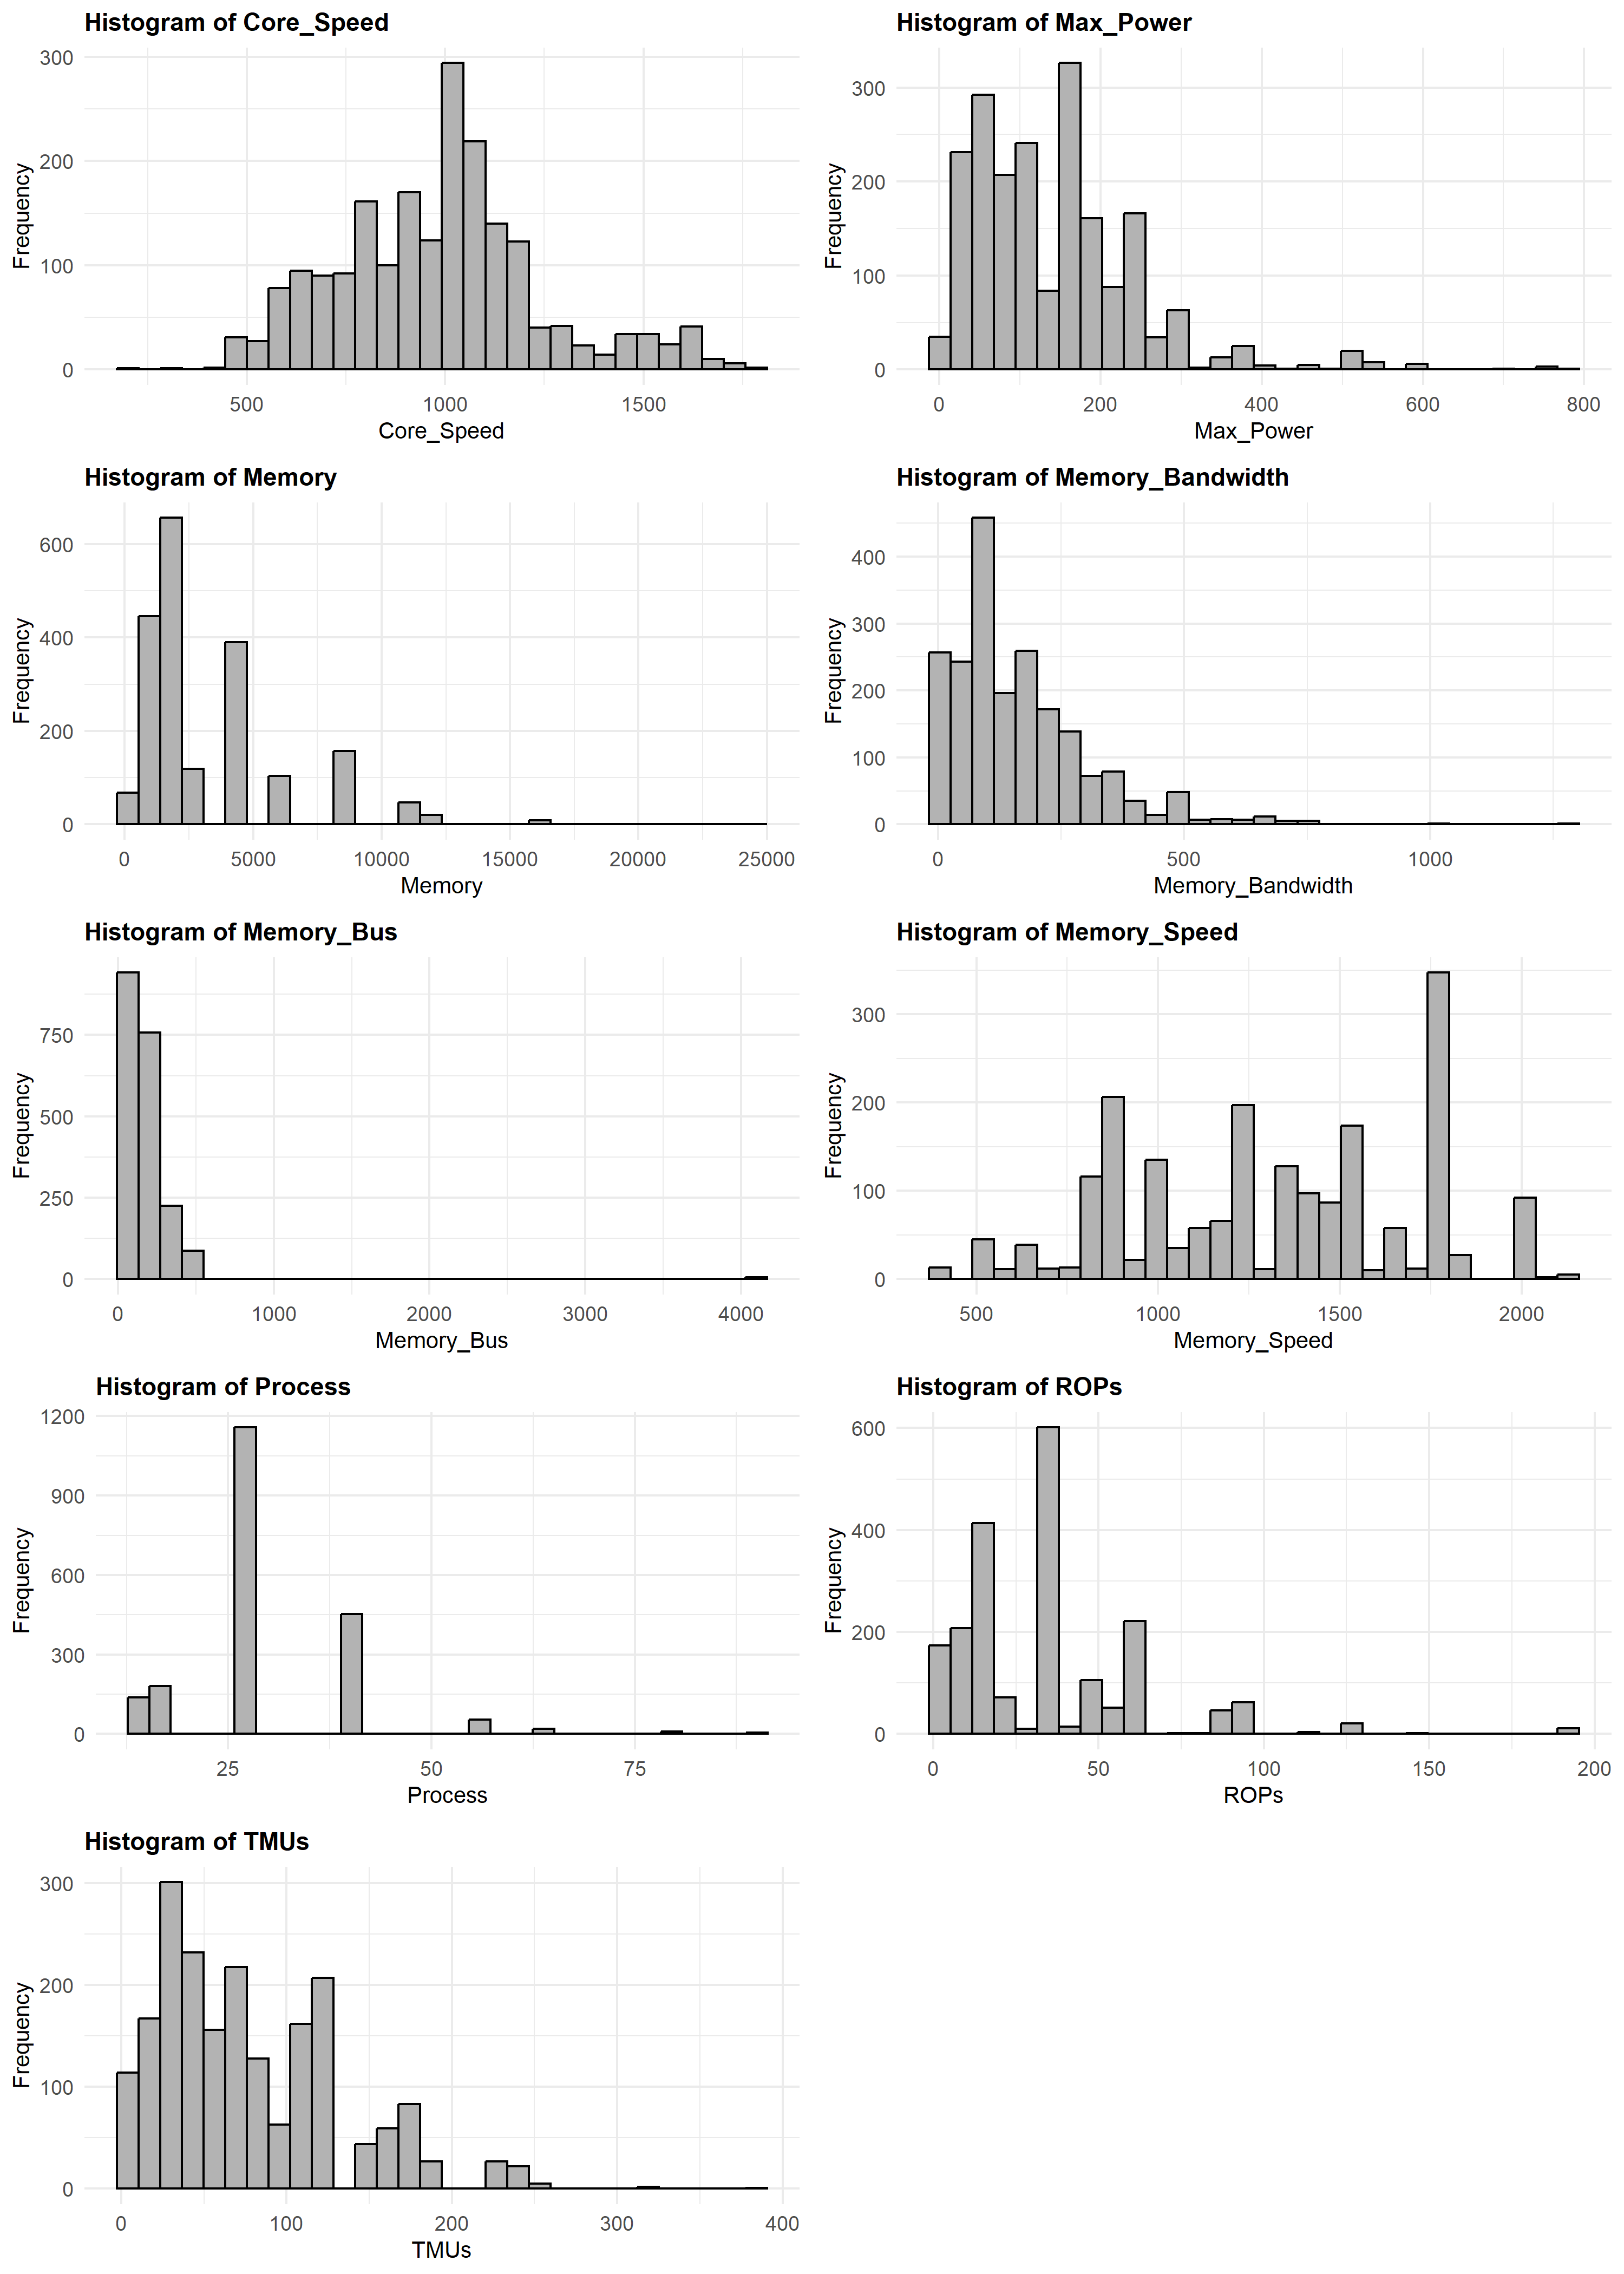
\includegraphics[width=0.92\textwidth]{statisticDes/histograms_original.png}
                \caption{Biểu đồ Histogram của các biến ở dạng dữ liệu gốc}
                \label{fig:hist_original_r5}
            \end{figure}

            \begin{figure}[H]
                \centering
                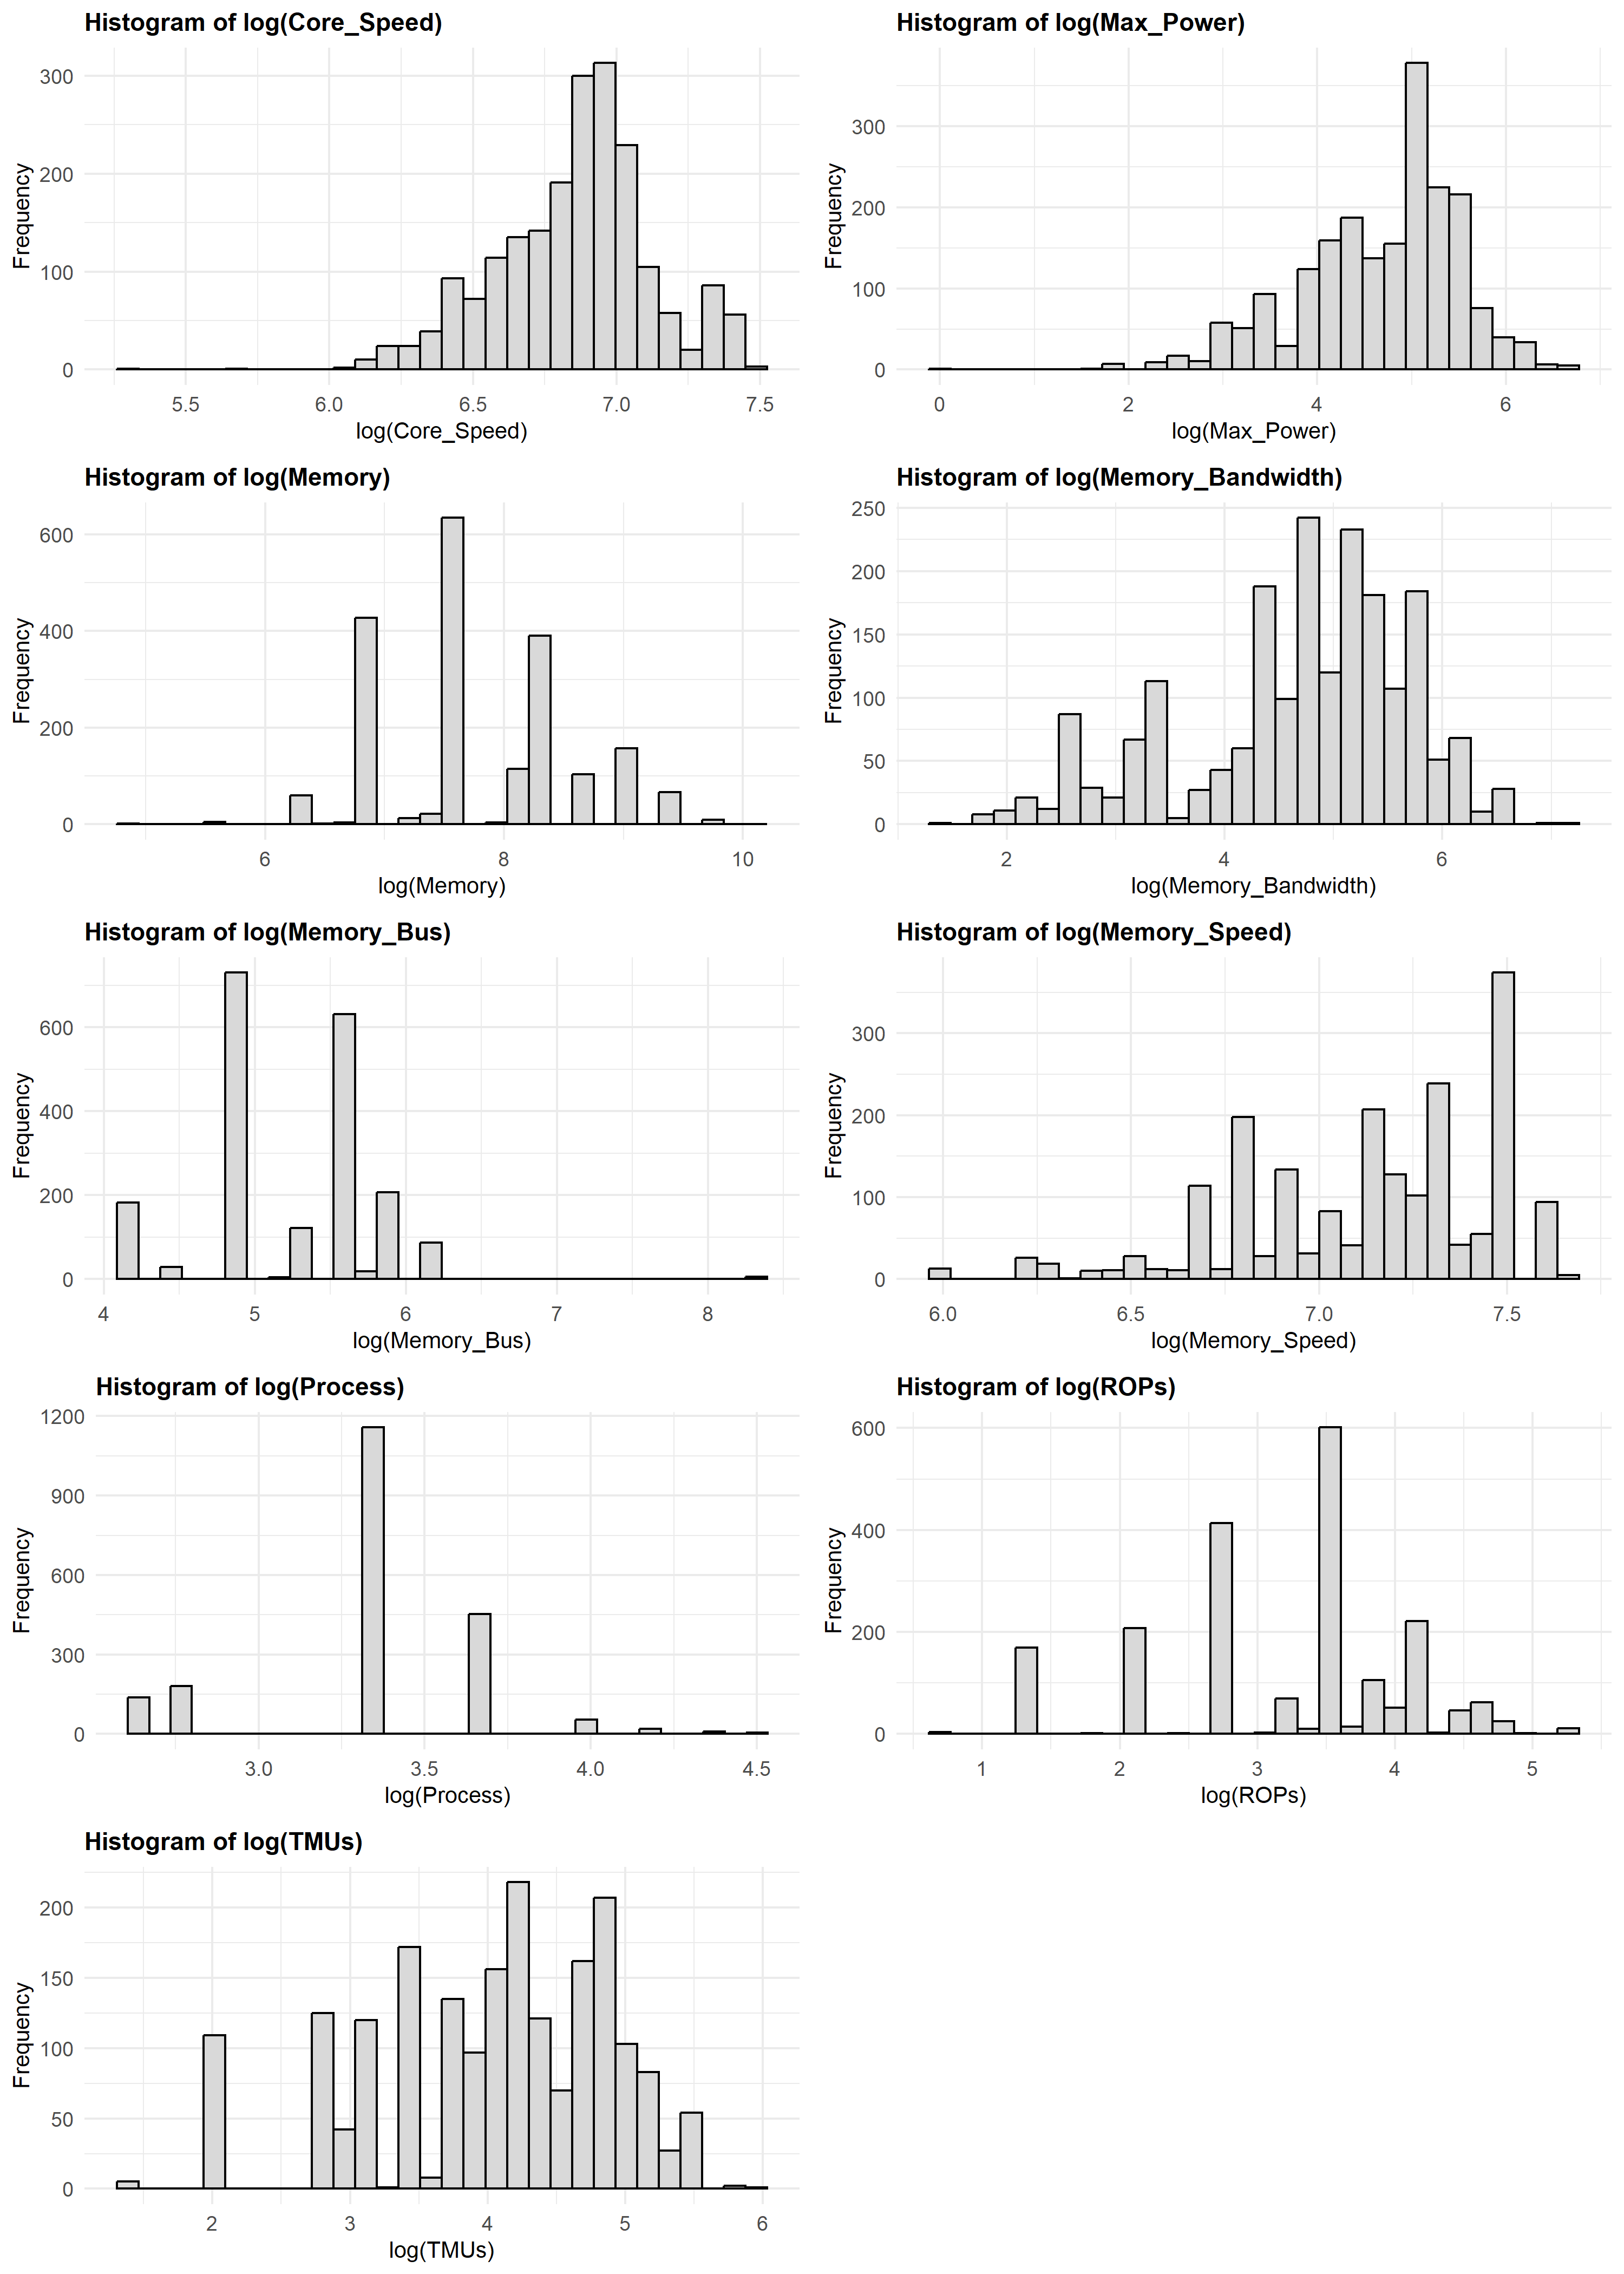
\includegraphics[width=0.92\textwidth]{statisticDes/histograms_log.png}
                \caption{Biểu đồ Histogram của các biến sau khi chuyển đổi sang dạng logarit}
                \label{fig:hist_log_r5}
            \end{figure}

            \textbf{Nhận xét về phân bố dữ liệu:}
            \begin{itemize}
                \item Ở dạng dữ liệu gốc (Hình \ref{fig:hist_original_r5}), hầu hết các biến phần cứng như \texttt{Memory}, \texttt{Memory\_Bandwidth}, \texttt{Max\_Power}, \texttt{ROPs}, và \texttt{TMUs} đều thể hiện độ lệch phải mạnh (Right-skewed distribution). Phần lớn các dòng GPU phổ thông tập trung ở khoảng giá trị nhỏ đến trung bình, trong khi một số ít GPU cao cấp nằm ở dải giá trị rất lớn.
                \item Sau khi áp dụng phép chuyển đổi logarit (Hình \ref{fig:hist_log_r5}), độ lệch của các biến được giảm đáng kể, phân bố dữ liệu trở nên đối xứng hơn và tiệm cận dạng phân phối chuẩn. Điều này giúp ổn định phương sai và đáp ứng tốt hơn các giả định của mô hình hồi quy tuyến tính ở các phần sau.
            \end{itemize}

        \subsubsection{Biểu đồ phân tán (Scatter Plot)}
            Để đánh giá mối quan hệ giữa biến phụ thuộc \texttt{log(Core\_Speed)} và các biến độc lập còn lại, nhóm tiến hành vẽ các biểu đồ phân tán dạng log bằng R:

            \begin{figure}[H]
                \centering
                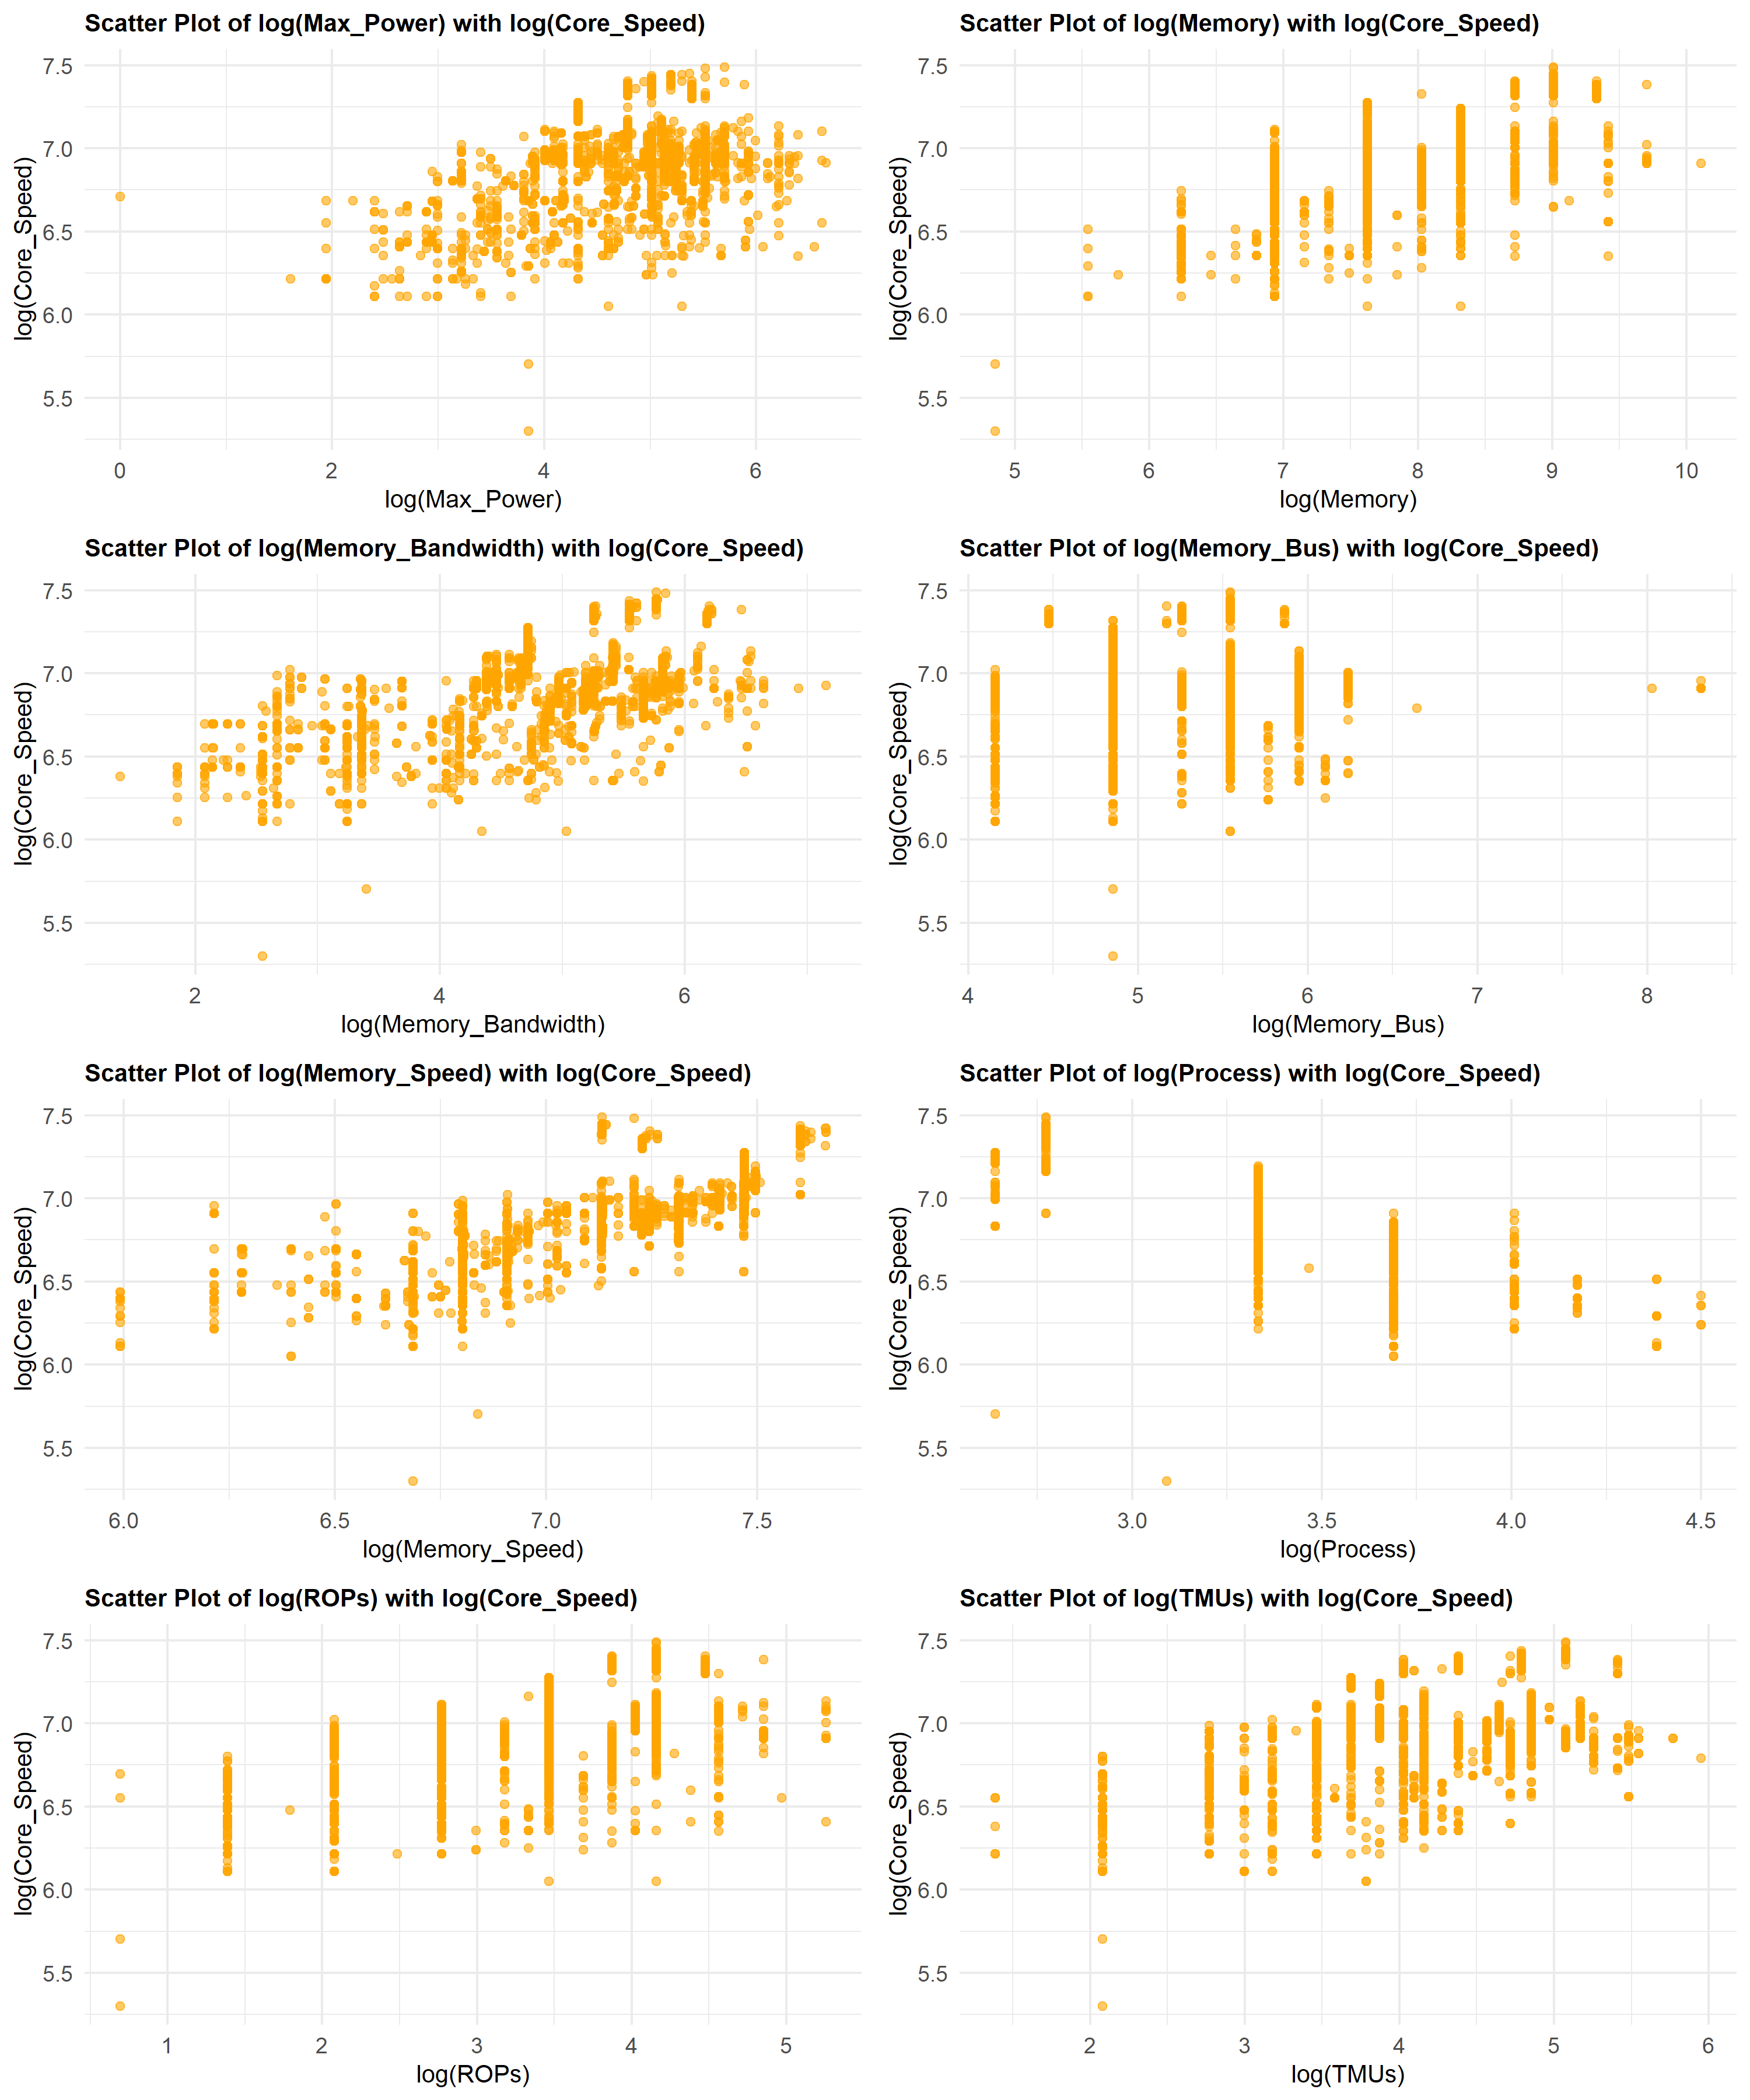
\includegraphics[width=0.92\textwidth]{statisticDes/scatter_log.png}
                \caption{Biểu đồ phân tán (Scatter Plot) giữa các biến độc lập với log(Core\_Speed)}
                \label{fig:scatter_log}
            \end{figure}

            \textbf{Nhận xét về mối quan hệ giữa các biến:}
            \begin{itemize}
                \item Dựa vào đồ thị phân tán giữa các biến \texttt{log(Max\_Power)}, \texttt{log(Memory\_Bandwidth)}, \texttt{log(Memory\_Speed)}, \texttt{log(Memory)}, \texttt{log(ROPs)}, \texttt{log(TMUs)} với \texttt{log(Core\_Speed)}, ta thấy mối quan hệ giữa các biến này với \texttt{log(Core\_Speed)} chủ yếu là \textbf{đồng biến} và phân tán với mật độ tương đối dày đặc.
                \item Đối với biến \texttt{log(Process)} (tiến trình sản xuất, nm), ta quan sát thấy xu hướng \textbf{nghịch biến} so với \texttt{log(Core\_Speed)}: công nghệ tiến trình nm càng nhỏ (bán dẫn càng tiên tiến) thì xung nhịp nhân \texttt{Core\_Speed} đạt được càng cao.
                \item Mối quan hệ dạng logarit thể hiện xu hướng tuyến tính rõ ràng hơn so với dữ liệu gốc, tạo tiền đề thuận lợi cho việc xây dựng mô hình hồi quy tuyến tính bội ở Phần 6.
            \end{itemize}